\documentclass[a4paper,11pt]{article}

%---Packages utilisés
\usepackage[utf8]{inputenc}
\usepackage[T1]{fontenc}
\usepackage[frenchb]{babel}
\usepackage{indentfirst}
\usepackage[]{graphicx}
\usepackage{amsmath}
\usepackage{ccaption}
\usepackage{vmargin}
\usepackage{textcomp}
\usepackage{fancyhdr}
%\usepackage[avantgarde]{quotchap}
\usepackage[Lenny]{fncychap}
\usepackage{cite}
\usepackage{siunitx}

\fancypagestyle{plain}{
\fancyhead[]{}
\fancyfoot[R]{\thepage}
\renewcommand{\headrulewidth}{0pt}}

%---Nouvelles commandes
\newcommand{\arronax}{\textsc{Arronax}}
\newcommand{\cyrce}{\textsc{Cyrcé}}
\newcommand{\Root}{\textsc{Root}}
\renewcommand{\baselinestretch}{1.2}

%\renewcommand{\chaptermark}[1]{%
% \markboth{\thechapter . \ #1}{}}

%---Mise en page
\setlength{\parindent}{2ex}
%\pagestyle{fancy}

%---Début du document
\begin{document}

%---Marges du document
\setmarginsrb{3.5cm}{1.5cm}{1.5cm}{2cm}{2ex}{3ex}{2ex}{5ex}
%1 est la marge gauche
%2 est la marge en haut
%3 est la marge droite 
%4 est la marge en bas
%5 fixe la hauteur de l'etête
%6 fixe la distance entre l'entte et le texte
%7 fixe la hauteur du pied de page
%8 fixe la distance entre le texte et le pied de page
%
%\chapterstyle{veelo}
%\renewcommand{\sectionmark}[1]{\markright{\thesection\ #1}}
\lhead[]{}
\fancyfoot[C]{}
\fancyfoot[R]{\thepage}

%%%%%%%%%%%%%%%%
\begin{center}
\subsection*{Analyse des données issues des irradiations sur \arronax\ (Juin 2017)}
\end{center}

\subsection*{Description des manips}
Dosion a été placé sur un banc mécanique pouvant le rapprocher ou l'éloigner par translation du bout de la ligne faisceau (cf. figure \ref{fig:manip}).
Ce banc offre une amplitude de déplacement allant de 0 cm à 60 cm.\\
Plusieurs mesures, énumérées dans le tableau \ref{tab:bilan}, ont ainsi été réalisées suivant des positions et des intensités différentes sous des faisceaux de protons de 68 MeV.
La notation \textit{trav.} signifie que la mesure a été réalisée alors que le banc regagnait sa position initiale.
Le mouvement s'est donc effectué de 65 cm à 5 cm vers le bout de ligne.

\begin{figure}[h]
\begin{center}
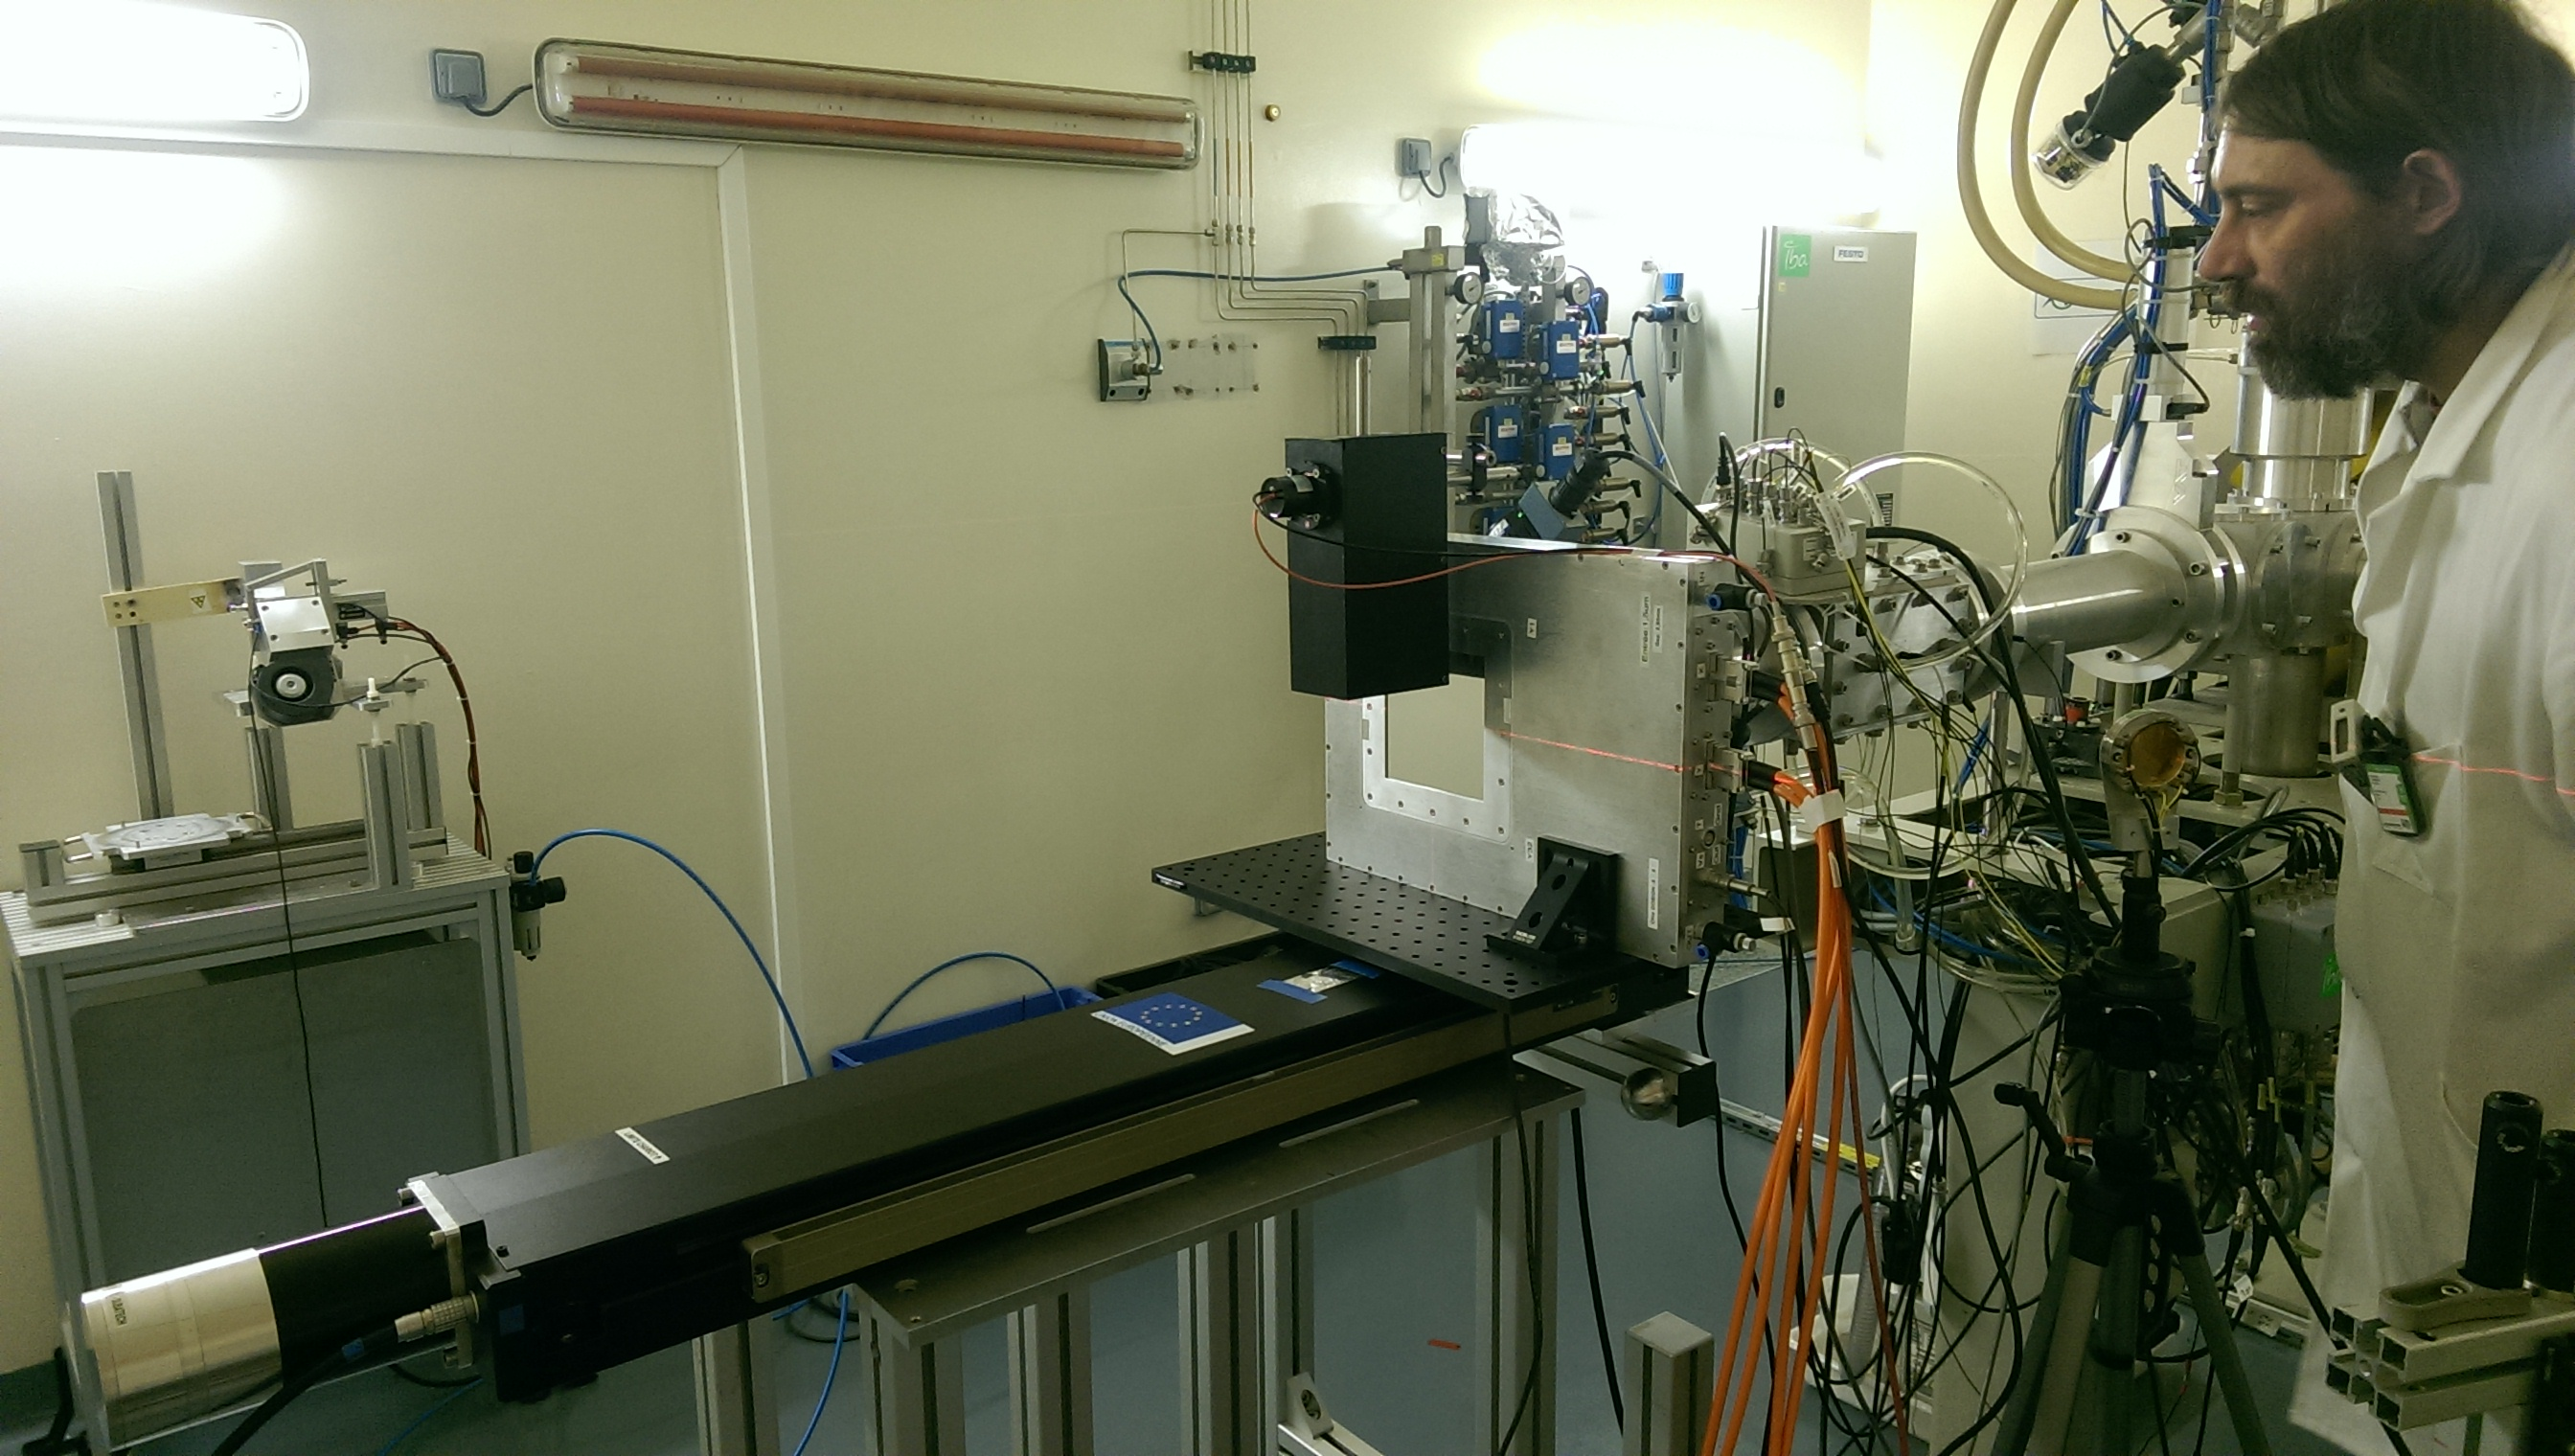
\includegraphics[width=0.8\linewidth]{Manip.jpg} 
\caption{\label{fig:manip}\footnotesize{Disposition du détecteur Dosion sur la ligne \arronax }}
\end{center}
\end{figure}

\begin{table}[h]
\begin{center}
\begin{tabular}{lr|lr|lr|r}
Fichier&nA&Fichier&nA&Fichier&nA&pos.\\
\hline
\hline
Acq\_1\_5cm\_1nA&1.0&Acq\_1\_5cm\_500A&0.5&Acq\_1\_5cm\_2nA&2.0&5 cm\\
Acq\_1\_17cm\_1nA&1.0&Acq\_1\_17cm\_500pA&0.5&Acq\_1\_17cm\_2nA&2.0&17 cm\\
Acq\_1\_29cm\_1nA&1.0&Acq\_1\_29cm\_500pA&0.5&Acq\_1\_29cm\_2nA&2.0&29 cm\\
Acq\_1\_41cm\_1nA&1.0&Acq\_1\_41cm\_500pA&0.5&Acq\_1\_41cm\_2nA&2.0&41 cm\\
Acq\_1\_53cm\_1nA&1.0&Acq\_1\_53cm\_500pA&0.5&Acq\_1\_53cm\_2nA&2.0&53 cm\\
Acq\_1\_65cm\_1nA&1.0&Acq\_1\_65cm\_500pA&0.5&Acq\_1\_65cm\_2nA&2.0&65 cm\\
Acq\_1\_trav\_1nA&1.0&Acq\_1\_trav\_500pA&0.5&Acq\_1\_trav\_2nA&2.0&trav.\\
\hline
\end{tabular}

\vspace{2ex}
\begin{tabular}{lrrl}
Fichier&fA&pos.&Notes\\
\hline
\hline
Calib\_1&200&5 cm&Calibrage avec PM\\
BI\_30fA&30&5 cm&Test à très basse intensité\\
\hline
\end{tabular}
\caption{\label{tab:bilan}\footnotesize{Ensemble des mesures réalisées}}
\end{center}
\end{table}

Les valeurs d'intensité sont approximatives dans le cas des mesures à différentes positions, et fournies par une seconde chambre d'ionisation placée avant Dosion pour les deux dernières acquisitions.

\subsection*{Résultat du calibrage}
Le calibrage réalisé a permis de sortir la valeur qui est utilisée pour l'ensemble des mesures étant donné qu'elles concernaient toutes des protons de 68 MeV.
Son analyse nous donne la valeur de :
$$Q/part = 0.0284 fC/part$$
Elle est très proche de la valeur théorique attendue de 0.0283 fC/part et nous permet notamment de recalculer l'intensité du faisceau, figure \ref{fig:intcalib}.

\begin{figure}[h]
\begin{center}
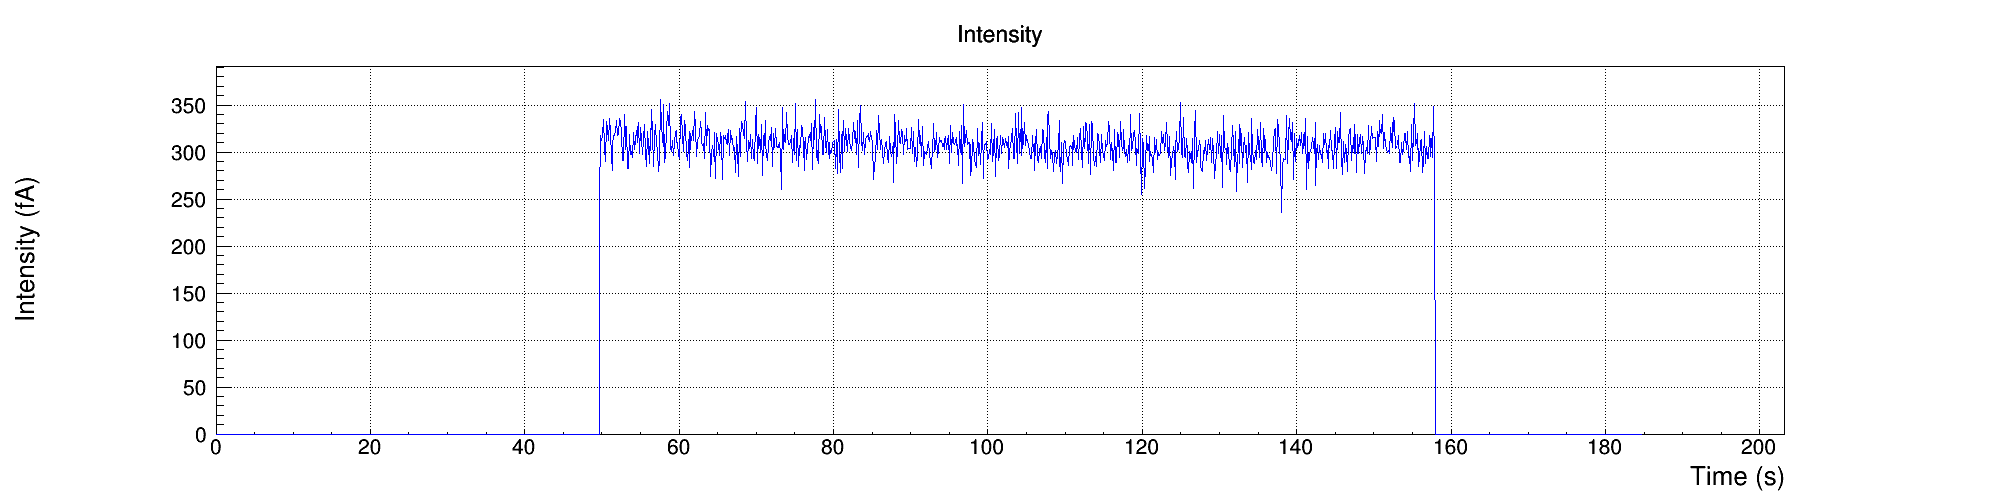
\includegraphics[width=1.\linewidth]{Intensity_calib.png} 
\caption{\label{fig:intcalib}\footnotesize{\'Evolution de l'intensité du faisceau au court de la mesure de calibrage}}
\end{center}
\end{figure}

Celle-ci est alors calculée à 300 fA ce qui diffère des 200 fA donnés par la première chambre d'ionisation. 

\subsection*{\'Ecartement du faisceau}
Tout comme pour la mesure de calibrage, l'intensité a été recalculée pour ces mesures à des valeurs moyennes de 13 pA pour la série 500 pA, 40 pA pour celle de 1 nA et 600 pA pour la dernière à 2 nA.
Les informations de 500 pA, 1 nA et 2 nA ayant été ajoutées uniquement à titre indicatif et sans réelle mesure précise avec la première chambre d'ionisation, cela explique des écarts aussi importants.

Un des principaux buts quant à l'utilisation du banc guidé est de voir l'évolution de la tache faisceau suivant la position de Dosion.
L'ajustement des profils en X et en Y se faisant par la somme de deux gaussiennes, c'est la largeur à mi-hauteur qui est comparée plutôt que l'écart-type.
Ils sont regroupés pour l'ensemble des irradiations, et suivant les axes X et Y, dans le tableau \ref{tab:fwhm}.
\begin{table}[h]
\begin{center}
\begin{tabular}{l|SSS|SSS}
&\multicolumn{3}{c|}{x (mm)}&\multicolumn{3}{c}{y (mm)}\\
Pos.&\multicolumn{1}{r}{500 pA}&\multicolumn{1}{r}{1 nA}&\multicolumn{1}{r|}{2 nA}&\multicolumn{1}{r}{500 pA}&\multicolumn{1}{r}{1 nA}&\multicolumn{1}{r}{2 nA}\\
\hline
\hline
5 cm&4.032&4.224&4.416&6.72&6.432&5.856\\
17 cm&4.704&4.8&5.28&7.584&7.2&6.72\\
29 cm&5.76&5.952&6.24&8.544&8.064&7.584\\
41 cm&7.2&7.296&7.104&9.504&8.928&8.448\\
53 cm&8.928&8.928&8.352&10.656&9.984&9.408\\
65 cm&10.752&10.656&9.696&11.712&11.04&10.56\\
\end{tabular}
\caption{\label{tab:fwhm}\footnotesize{\'Evolution des largeurs à mi-hauteur suivant les axes x et y pour chacune des irradiations}}
\end{center}
\end{table}
Ce que nous pouvons tout de suite remarquer c'est que le faisceau est plus large suivant l'axe y que suivant l'axe x, comme nous le remarquons sur la figure \ref{fig:analyse}.
\begin{figure}[h]
\begin{center}
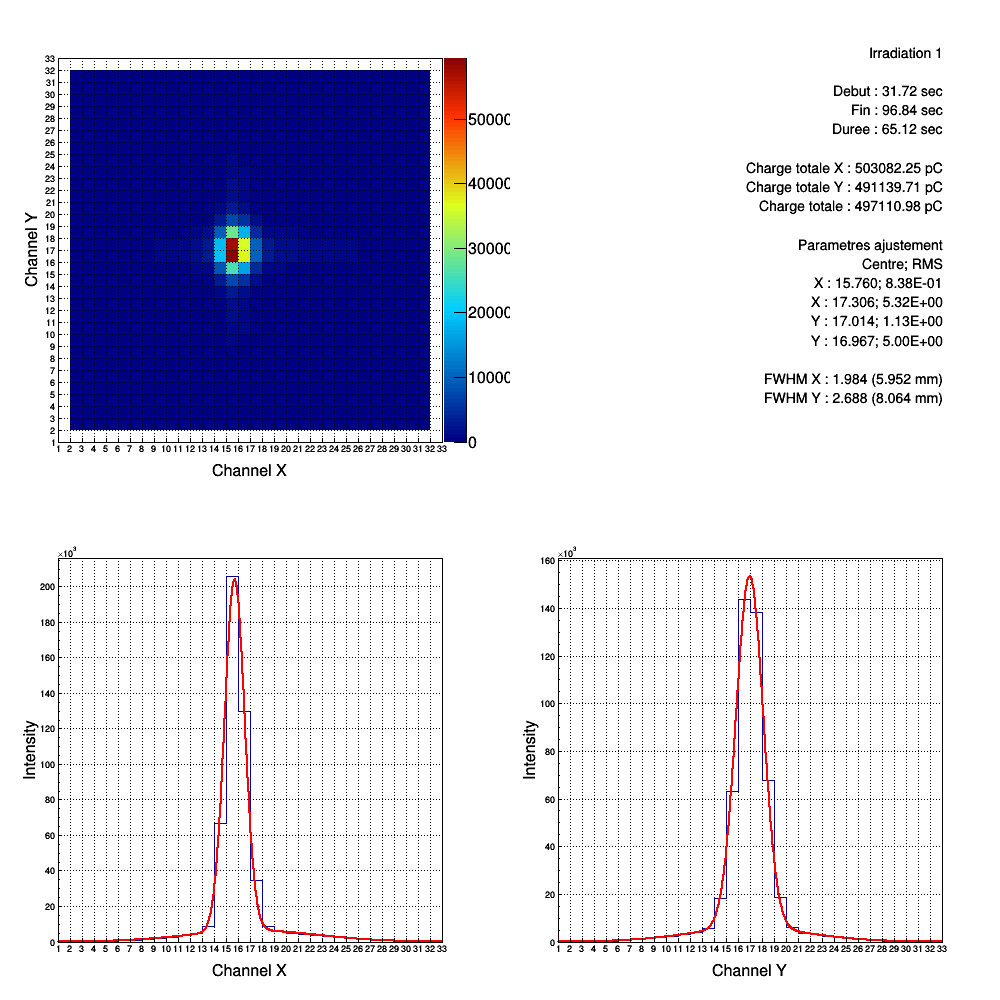
\includegraphics[width=1.\linewidth]{Area_1.png} 
\caption{\label{fig:analyse}\footnotesize{Résultats de l'analyse du fichier de mesure concernant l'irradiation à 29 cm et 1 nA.}}
\end{center}
\end{figure}

Concernant la comparaison des valeurs pour des distances identiques mais à des intensités différentes, il semblerait que les séries à 500 pA et 1 nA soient relativement proches tandis que nous notons quelques écarts pour la dernière à 2 nA.
C'est peut-être dû aux intensités réelles des mesures -- respectivement 13 pA, 40 pA et 600 pA -- qui montre que l'écart entre les deux premières et la dernière est beaucoup plus important.
 
\subsection*{Analyse en mouvement}
Dosion étant très sensible au bruit microphonique et aux vibrations, le mouvement du banc constitue une source de bruit très important comme en témoigne la figure \ref{fig:charge}.
La zone temporelle correspondant au déplacement du banc se devine très facilement par l'augmentation du bruit autour de la valeur moyenne.
\begin{figure}[h]
\begin{center}
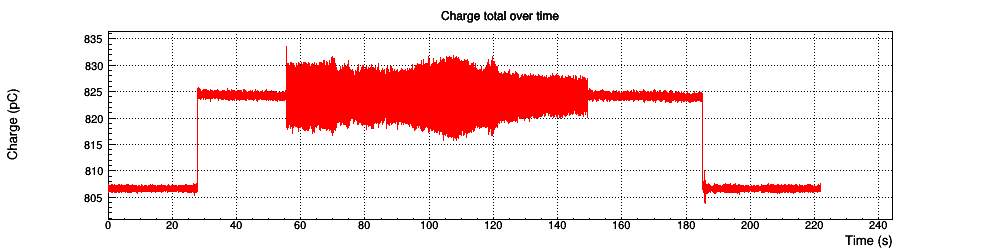
\includegraphics[width=1.\linewidth]{Charge.png} 
\caption{\label{fig:charge}\footnotesize{\'Evolution de la charge mesurée au cours du temps pour l'irradiation à 1 nA avec le banc en déplacement.}}
\end{center}
\end{figure}
Tout comme pour les données de Cyrcé, j'ai utilisé une soustraction du bruit de fond par ajustement trame par trame pour définir le zéro, figure \ref{fig:zero}, et ainsi permettre la correction que nous pouvons observer sur la figure \ref{fig:cclean}.
\begin{figure}[h]
\begin{center}
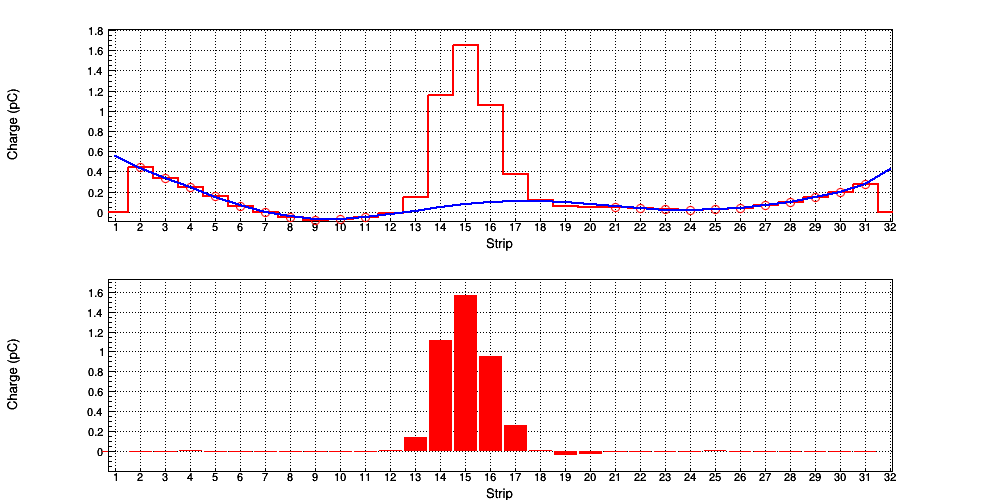
\includegraphics[width=1.\linewidth]{SFB_143.png} 
\caption{\label{fig:zero}\footnotesize{Exemple de correction du zéro en utilisant un ajustement trame par trame.}}
\end{center}
\end{figure}
\begin{figure}[h]
\begin{center}
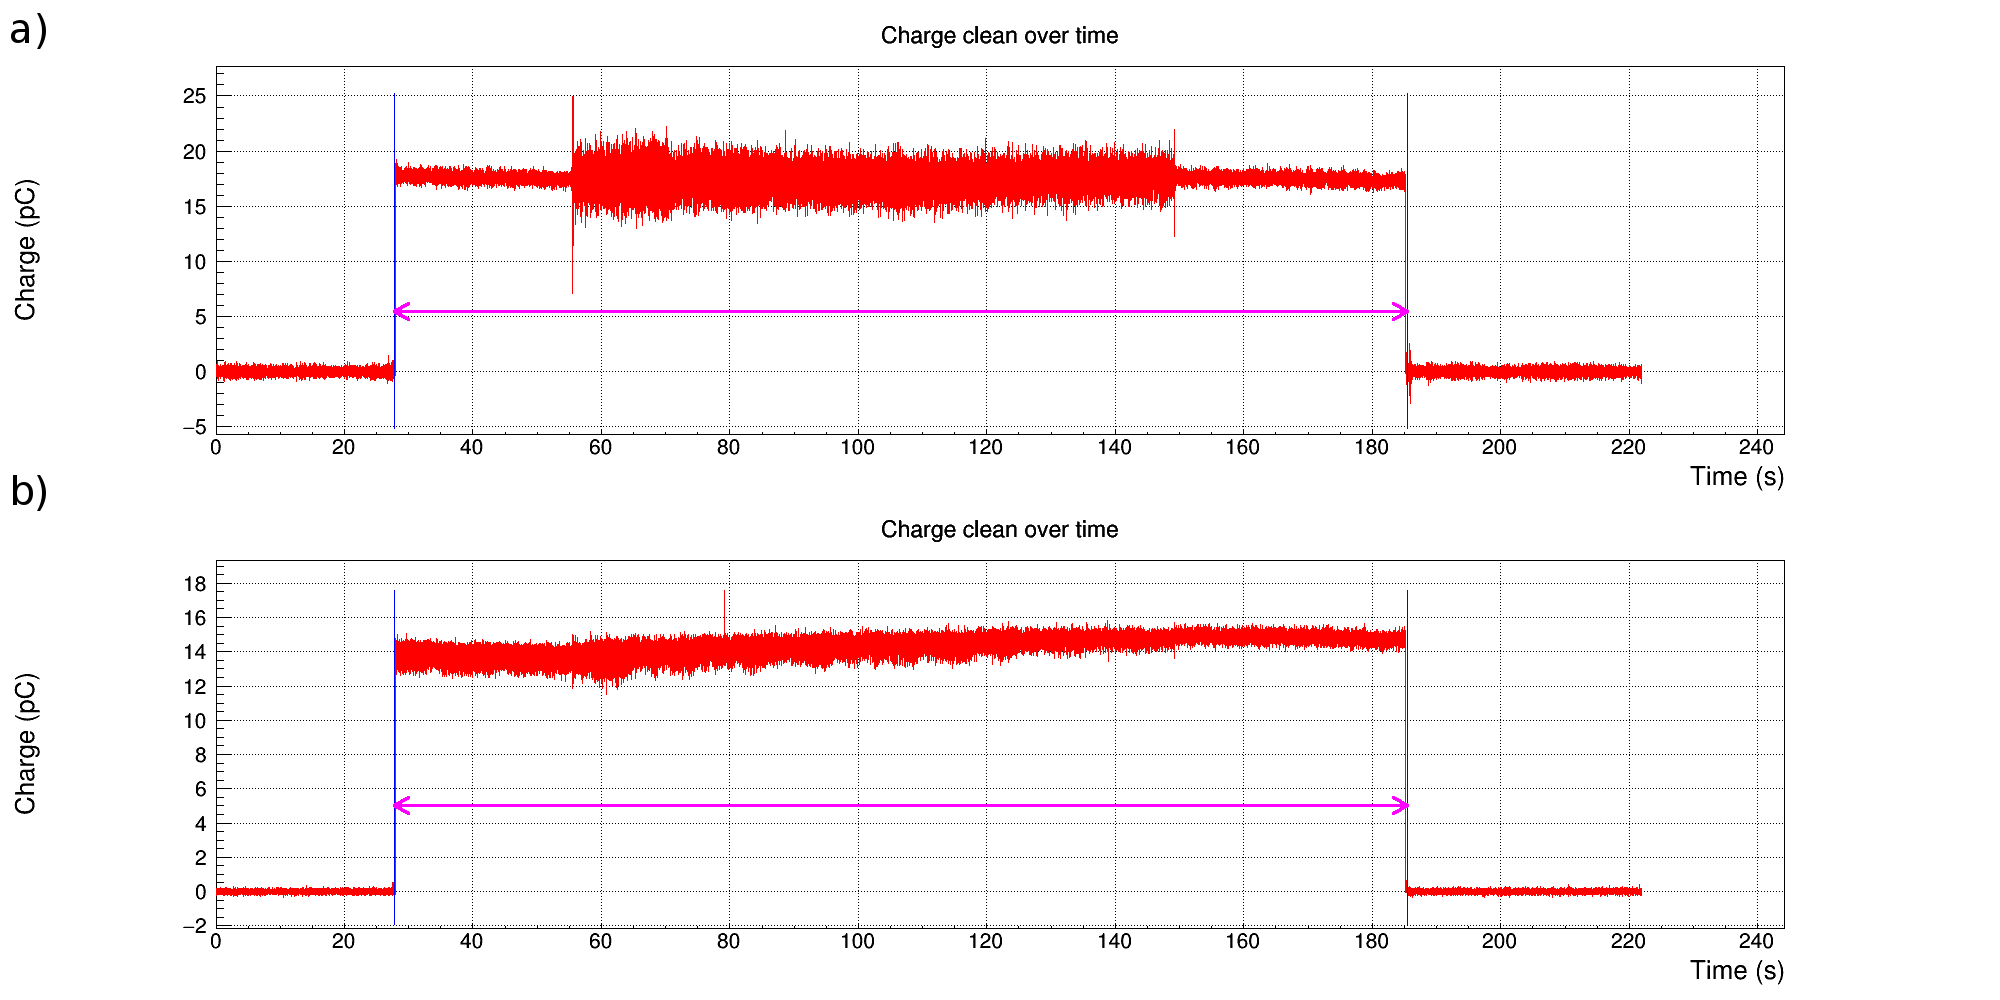
\includegraphics[width=1.\linewidth]{Charge_noclean.png} 
\caption{\label{fig:cclean}\footnotesize{a) Charge intégrale corrigée avec une soustraction par défaut du bruit de fond. b) Charge intégrale corrigée avec une soustraction trame par trame du bruit de fond.}}
\end{center}
\end{figure}

Avec ces acquisitions en mouvement nous pouvons observer l'évolution directe de l'écartement du faisceau comme dans le cas de l'irradiation à 500 pA sur la figure \ref{fig:trav_500pA}.
Le fait que l'écartement, et l'écart-type associé, diminue en fonction du temps est simplement dû au fait que le banc revenait de sa position la plus éloignée -- 65 cm -- à sa position la plus proche -- 5 cm.
\begin{figure}[h]
\begin{center}
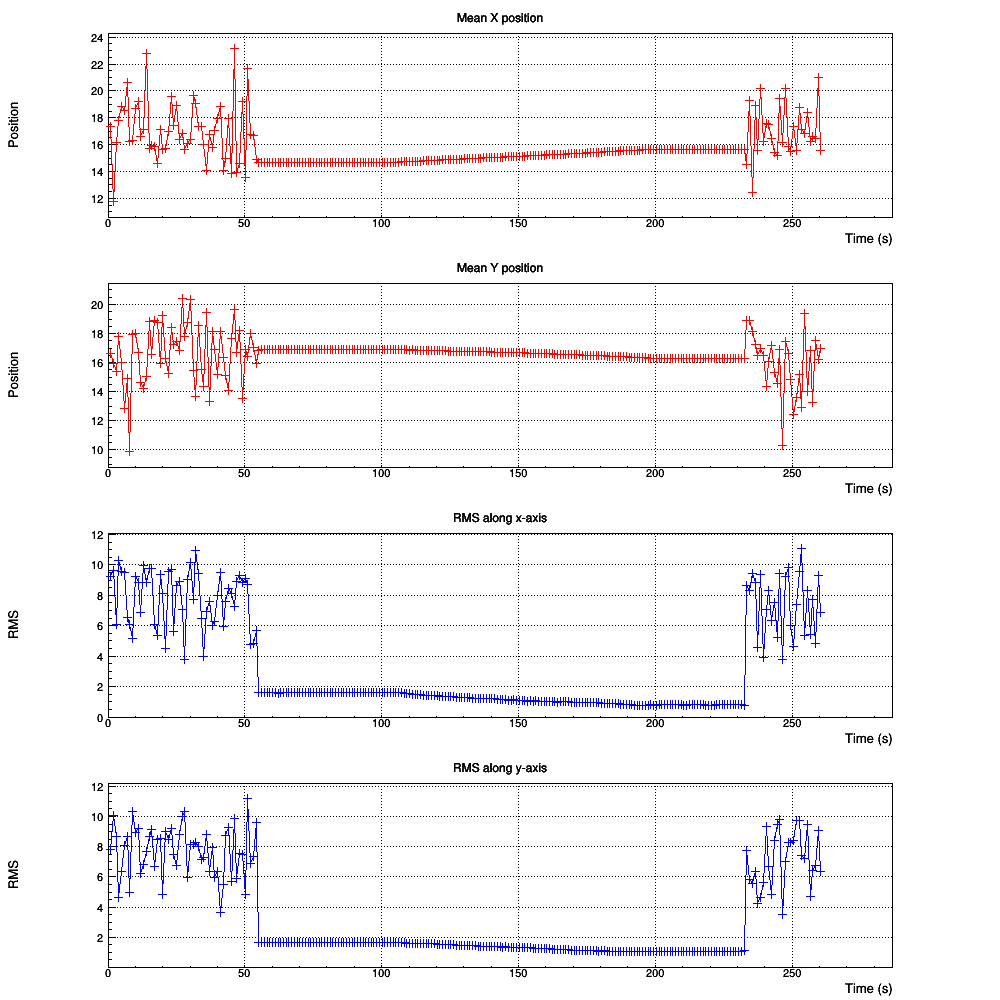
\includegraphics[width=1.\linewidth]{Trav_500pA.png} 
\caption{\label{fig:trav_500pA}\footnotesize{De haut en bas : Évolution de la position moyenne le long de l'axe X ; évolution de la position moyenne le long de l'axe Y ; évolution de l'écart-type en position le long de l'axe X ; évolution de l'écart-type en position le long de l'axe Y.}}
\end{center}
\end{figure}

\subsection*{Très faible intensité}
L'irradiation à 30 fA, indiqués par la première chambre d'ionisation, avait pour but d'éprouver la méthode d'analyse à très faible intensité.
Nous remarquons qu'étant à faible intensité, la chambre est plus sensible aux perturbations extérieures, comme le bruit, et que des fluctuations trop importantes, visibles sur la figure \ref{fig:bi} entre 220 sec et 270 sec, nous empêchent de réaliser une analyse cohérente sur toute la période d'irradiation, s'étendant de 30 sec à 270 sec.
\begin{figure}[h]
\begin{center}
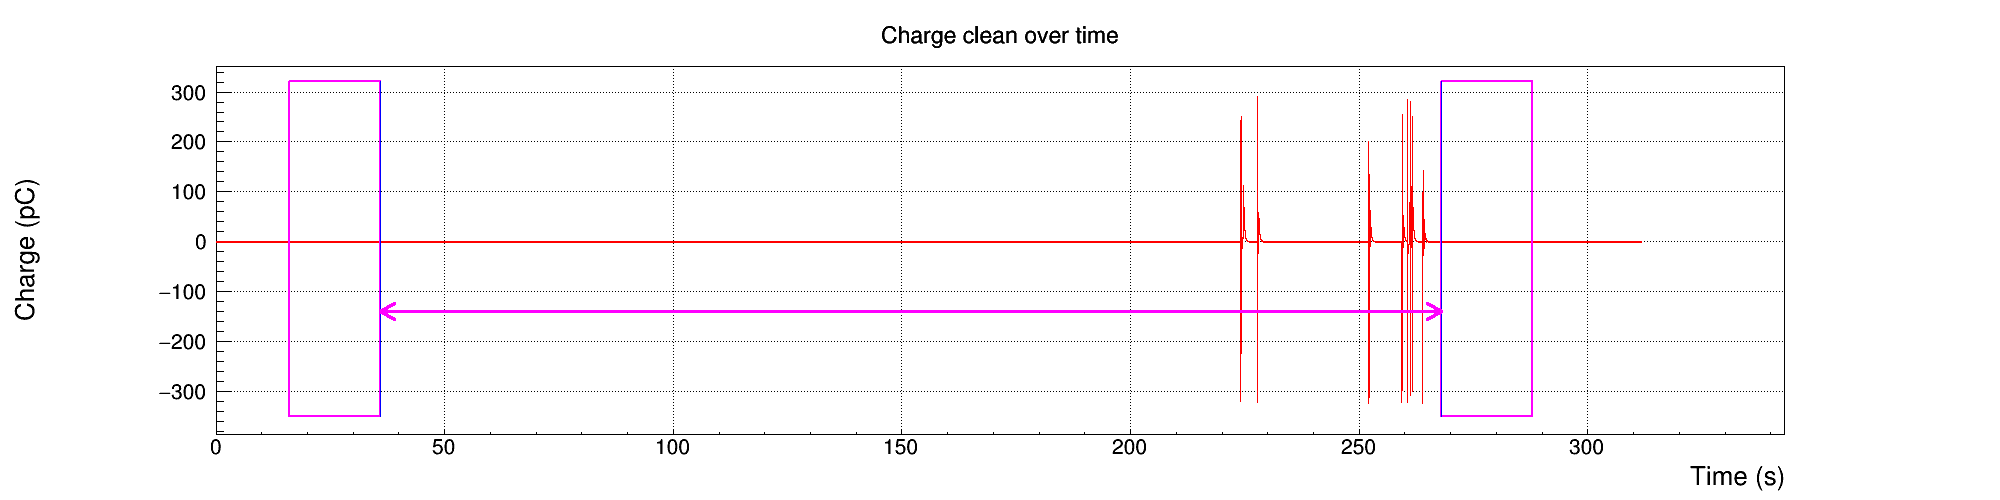
\includegraphics[width=1.\linewidth]{Perturbations.png} 
\caption{\label{fig:bi}\footnotesize{Charge totale obtenue lors de l'irradiation à très basse intensité.}}
\end{center}
\end{figure}

Pour s'affranchir de ce problème, nous procédons à une analyse à deux passes ; durant le premier passage nous fixons manuellement les bornes d'irradiation à 30 sec et 270 sec, les "véritables" valeurs, pour ainsi calculer le bruit de fond ; et lors de second passage, nous restreignons la zone d'étude sur une plage sans perturbation, de 50 sec à 200 sec, et nous procédons à son analyse en utilisant la valeur du bruit de fond calculée lors du premier passage.
Cela nous permet donc d'obtenir les résultats présentés sur la figure \ref{fig:bianalyse}. 
\begin{figure}[h]
\begin{center}
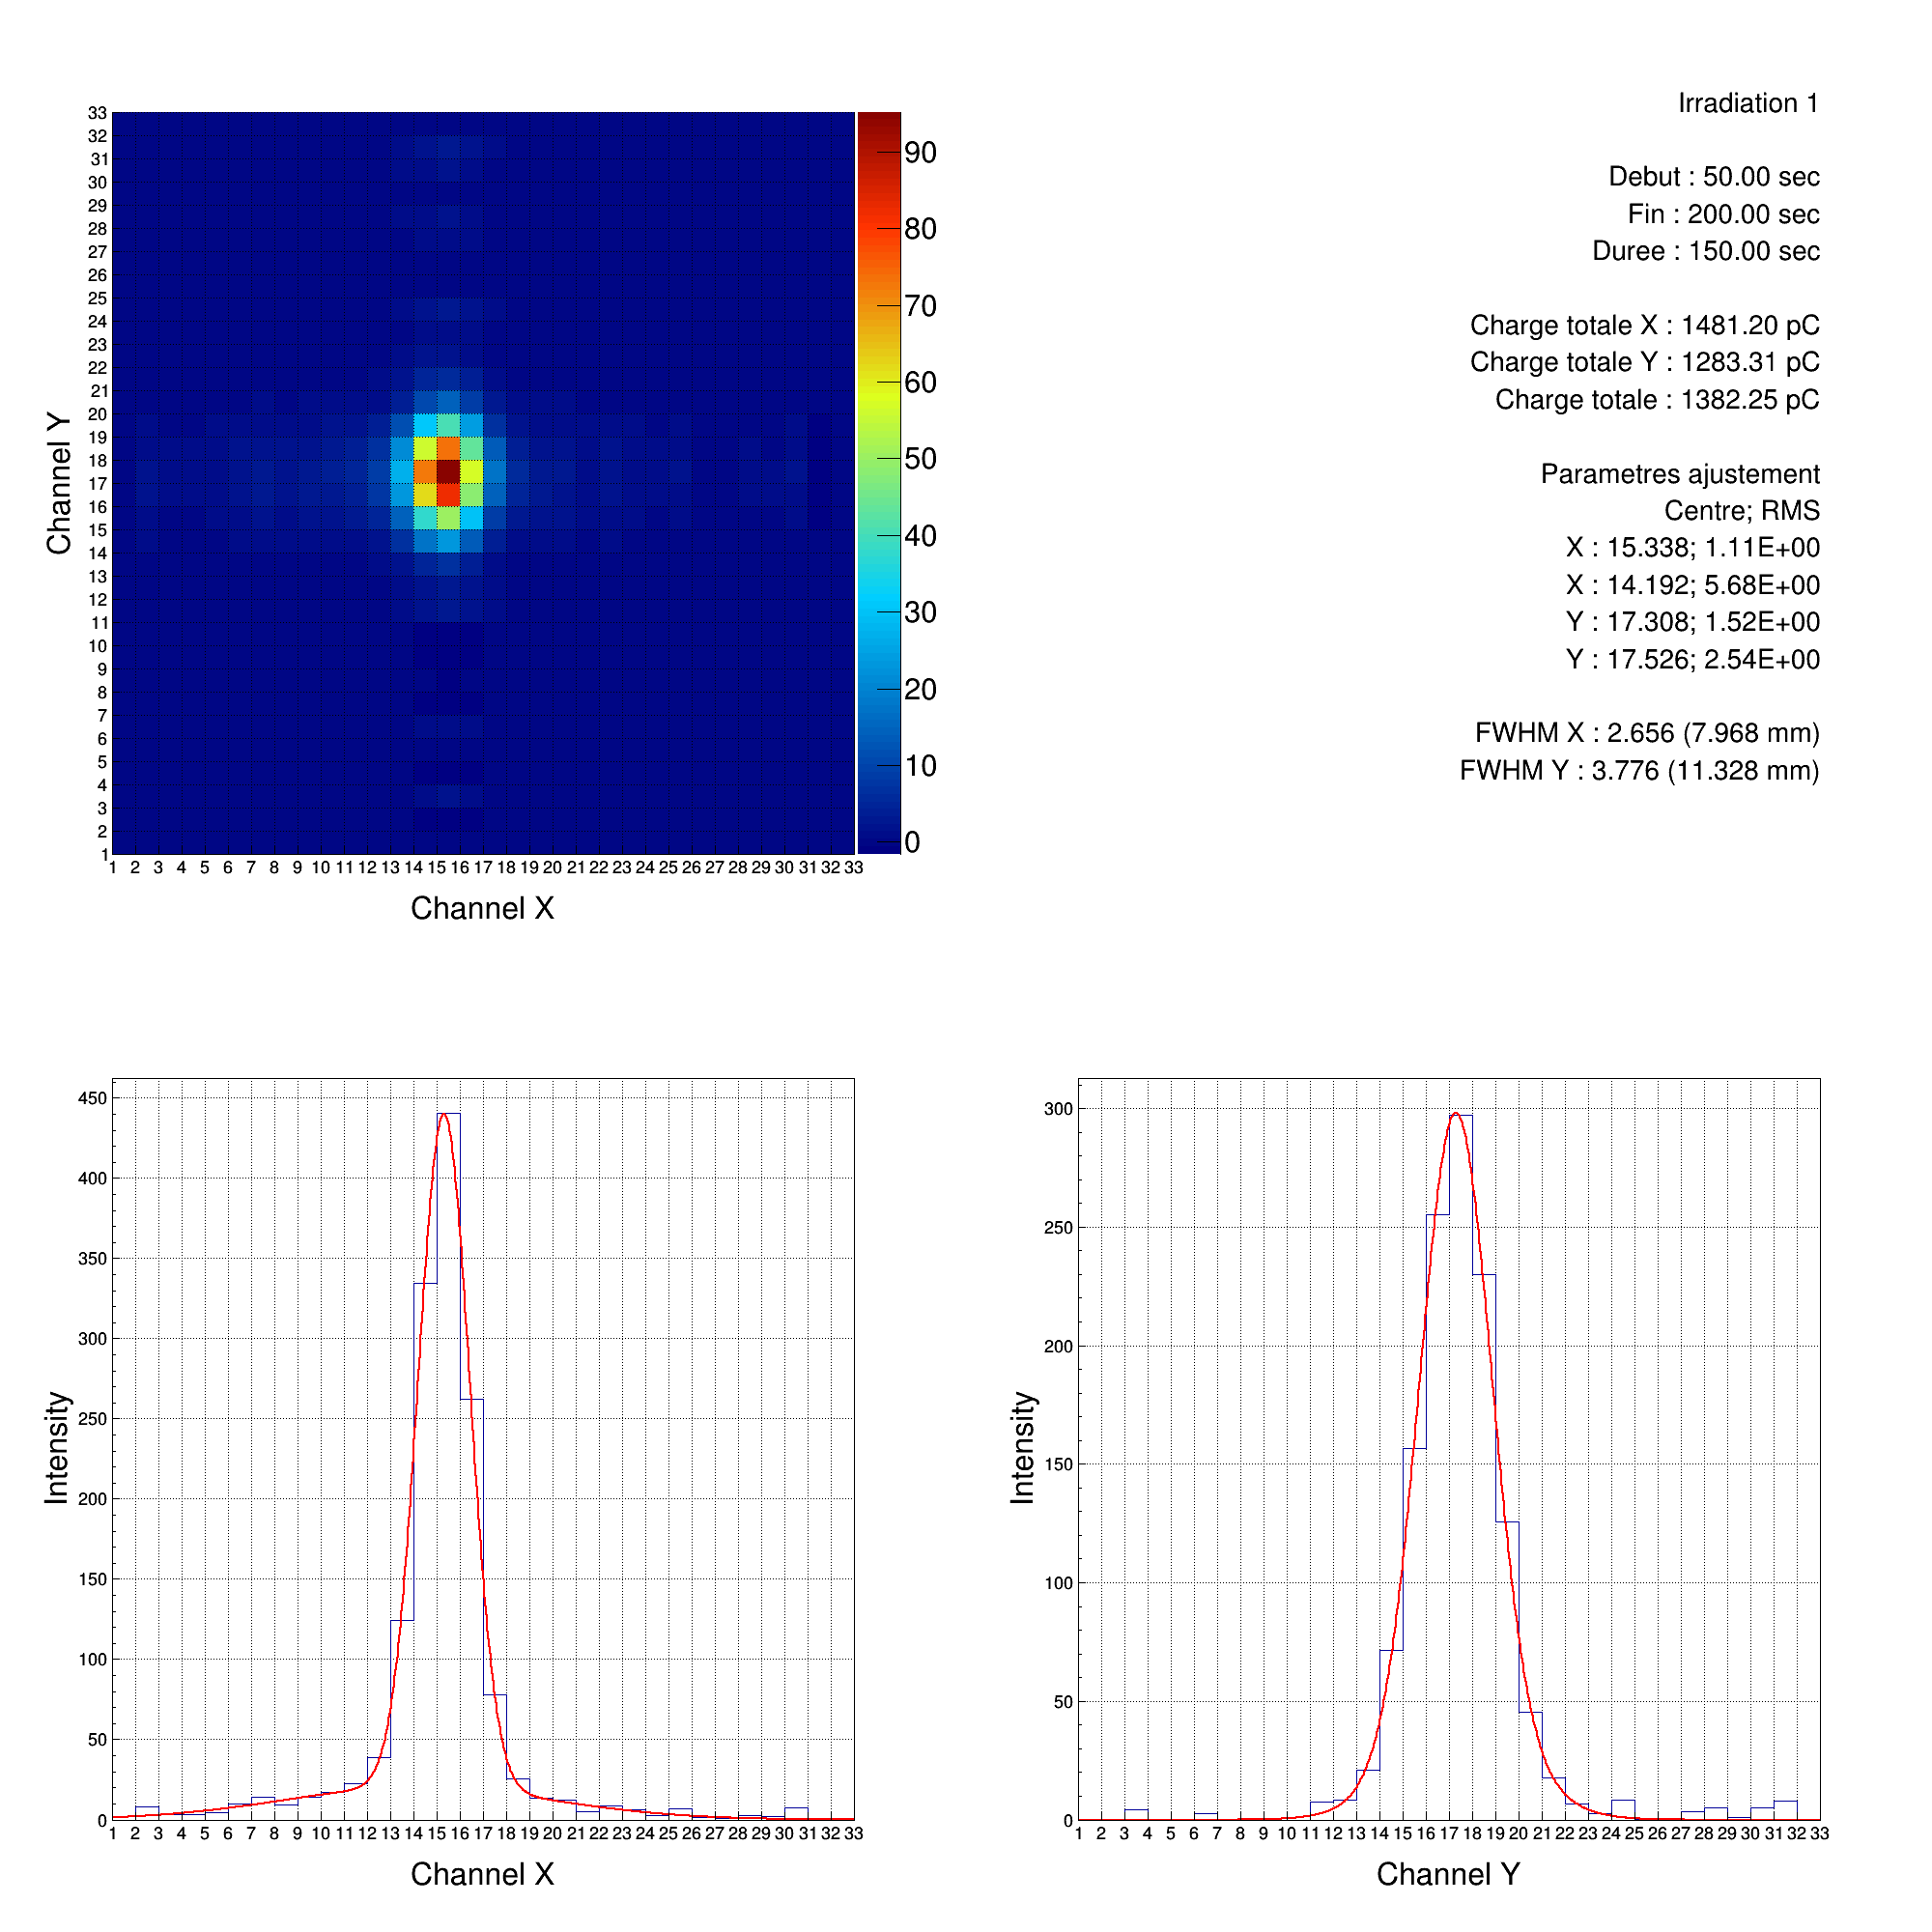
\includegraphics[width=1.\linewidth]{Area_1_bi.png} 
\caption{\label{fig:bianalyse}\footnotesize{Résultats de l'analyse du fichier de mesure concernant l'irradiation à très basse intensité.}}
\end{center}
\end{figure}

Comme pour les autres irradiations où les valeurs indicatives d'intensité -- 500 pA, 1 nA et 2 nA -- ont été recalculées à partir du résultat du calibrage -- respectivement 13 pA, 40 pA et 600 pA -- dans ce cas là nous passons des 30 fA, donnés par la première chambre, à 50 fA, figure \ref{fig:biintensity}.
\begin{figure}[h]
\begin{center}
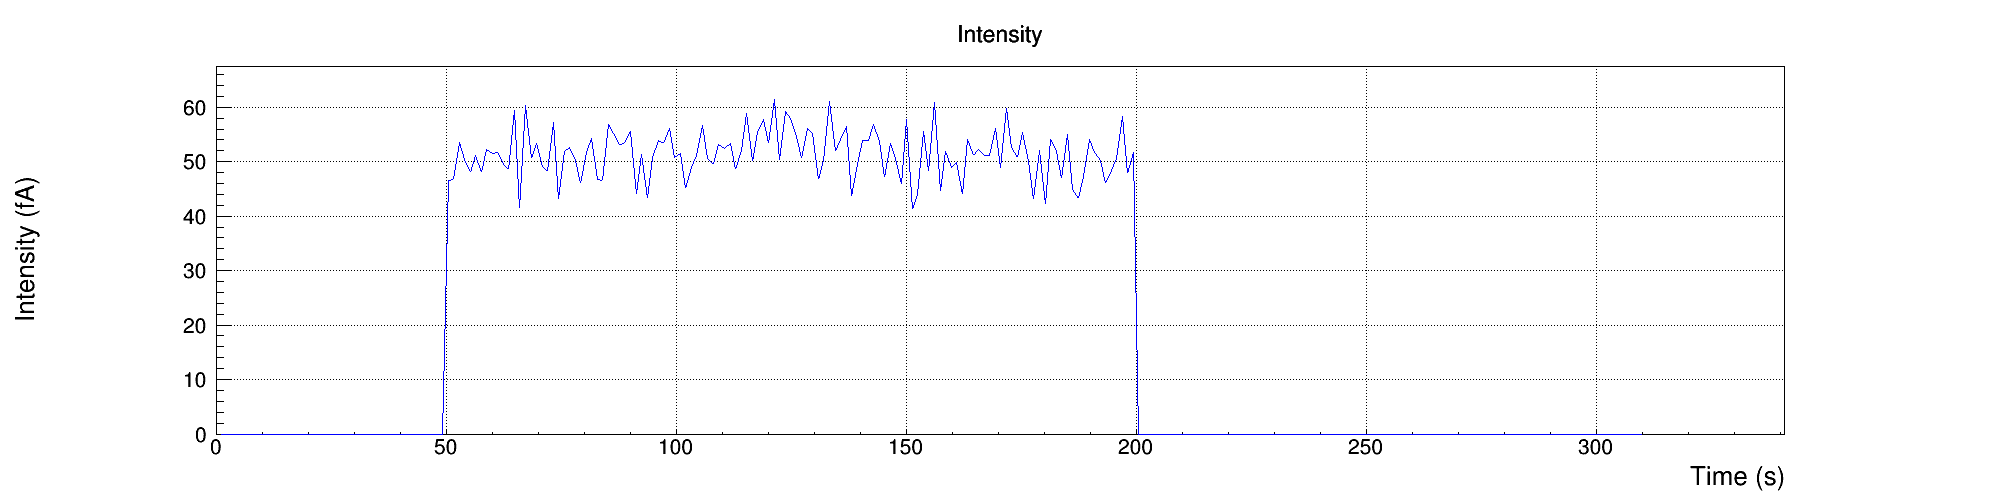
\includegraphics[width=1.\linewidth]{Intensity_clean.png} 
\caption{\label{fig:biintensity}\footnotesize{Intensité obtenue lors de l'irradiation à très basse intensité.}}
\end{center}
\end{figure}

%%%%%%%%%%%%%%%%%%%%%%%%%%%%%%%%%%

\end{document}

%%%%%%%%%%%%%%%%%%%%%%%%%%%%%%%%%%%%%%%%%%%%%%%%%%%%%%%%%%%%%%%%%%%%%%%%%%%%%%%%%%%%%%%%%%%%%%%%%%